\documentclass[12 pt, a4paper]{report}
\usepackage[utf8]{inputenc}

\usepackage{natbib}
\usepackage{graphicx}
\usepackage[toc]{appendix}
\usepackage{titlesec}
\usepackage{fancyhdr}
\usepackage{listings}

\renewcommand{\contentsname}{Table des matières}
\renewcommand{\listfigurename}{Liste des figures}
\renewcommand{\listtablename}{Liste des tableaux}
\renewcommand{\appendixname}{Annexe}
\renewcommand{\appendixtocname}{Annexes}

%% NUMÉROS DE PAGE

\fancyhf{} % clear all header and footers
\renewcommand{\headrulewidth}{0pt} % remove the header rule
\rhead{\thepage}
\pagestyle{fancy}

\makeatletter % Un hack pour les numéros de page
\renewcommand\chapter{\if@openright\cleardoublepage\else\clearpage\fi
                    \thispagestyle{fancy}%
                    \global\@topnum\z@
                    \@afterindentfalse
                    \secdef\@chapter\@schapter}
\makeatother

%% TITRES

%hang block display runin
% straight: titre un après l'autre, mettre \pagebreak pour sauter de page
\renewcommand{\chaptername}{}
\titleclass{\chapter}{straight}
\titleformat{\chapter}
[hang]
{\raggedright\normalfont\Large\bfseries}
{\filright\MakeUppercase{\chaptertitlename} \Large\thechapter\ - }
{0pt}
{\Large\MakeUppercase}

%% ------------------------- variables ---------------------------------

\newcommand\var[2]{\newcommand{#1}{\ensuremath{#2}}}
\var\Fx{F_x}
\var\Fy{F_y}
\var\vF{\rm\bf F}
\var\Fmin{F_{\rm min}}
\var\Fmax{F_{\rm max}}

%% ------------------------ document commence --------------------------
\begin{document}

\begin{titlepage}
    \begin{center}
        \large
        DÉPARTEMENT DE GÉNIE MÉCANIQUE\\
        Faculté de génie\\
        Université de Sherbrooke\\
        
        \vspace{3cm}
 
        \Huge
        \textbf{Gabarit \LaTeX}
        
        \large
 
        \vspace{3cm}
 
        par\\
        Équipe 1\\
        TOMMY ALPHA\\
        TOMMY BETA\\
        TOMMY CHARLIE\\
        TOMMY DELTA\\
        TOMMY EPSILON\\
        TOMMY FARADAY\\
 
        \vfill
 
        Travail présenté à\\
        ORGANISATION
 
        \vspace{1.5cm}
 
        %\includegraphics[width=0.4\textwidth]{university}
 
        \Large
        Sherbrooke\\
        1 JANVIER 2019
 
    \end{center}
\end{titlepage}

\linespread{1.25} % Équivalent à interligne et demi de Word
\chapter*{Sommaire}
\pagebreak

\linespread{1} % Simple interligne
\tableofcontents
\pagebreak

\linespread{1.25} % Équivalent à interligne et demi de Word
\addcontentsline{toc}{chapter}{\listfigurename}
\listoffigures
\addcontentsline{toc}{chapter}{\listtablename}
\renewcommand{\tablename}{Tableau} % Table ou Tableau
\renewcommand{\thetable}{\arabic{table}}
\listoftables
% --------------------- LISTE DE VARIABLES ----------------------
\addcontentsline{toc}{chapter}{Liste de variables}
\chapter*{Liste de variables}

\begin{tabular}{ l l }
\Fx & La force en $x$\\
\Fy & La force en $y$\\
\Fmin & La force minimale\\
{$\theta$} & L'angle theta\\
\vF & Le vecteur de la force\\
\end{tabular}

\addcontentsline{toc}{chapter}{Liste d'abréviations}
\chapter*{Liste d'abréviations}
\pagebreak

\chapter{Introduction}
Ce document est un gabarit pour générer un document \LaTeX.

\pagebreak

\chapter{Problématique}
\chapter{Objectifs}

\pagebreak

\chapter{État des connaissances}
\section{Méthodologie}
\subsection{Sous-section}
\section{Résultats}

\chapter{Fonctions \LaTeX}

On déclare les variables au début. Après on peut les utiliser comme \Fx\ ou \Fy, ou encore \Fmax, ou encore le vecteur \vF. Mais est-ce que ça marche après dans une équation?

\begin{equation}
    \Fx{} = 0
\end{equation}

\begin{figure}[h!]
\centering
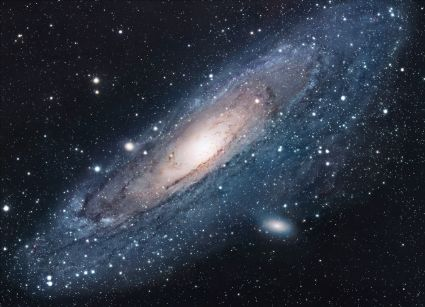
\includegraphics[scale=1.7]{universe}
\caption{The Universe}
\label{fig:universe}
\end{figure}

\chapter{Conclusion}
``I always thought something was fundamentally wrong with the universe'' \citep{adams1995hitchhiker}

\begin{appendices}
\chapter{Aide-mémoire des fonctions \LaTeX}
Voici des tables contenant les fontions \LaTeX les plus utilisés. La table \ref{table:1} présente les fonctions de traitement de textes. 
 
\begin{table}[h!]
\centering
\caption{Table to test captions and labels}
\begin{tabular}{||c c c c||} 
 \hline
 Col1 & Col2 & Col2 & Col3 \\ [0.5ex] 
 \hline\hline
 1 & 6 & 87837 & 787 \\ 
 2 & 7 & 78 & 5415 \\
 3 & 545 & 778 & 7507 \\
 4 & 545 & 18744 & 7560 \\
 5 & 88 & 788 & 6344 \\ [1ex] 
 \hline
\end{tabular}
\label{table:1}
\end{table}

\chapter{Fragments de code \LaTeX}

\newenvironment{boxed}
    {\begin{center}
    \begin{tabular}{|p{0.9\textwidth}|}
    \hline\\
    }
    { 
    \\\\\hline
    \end{tabular} 
    \end{center}
    }
%--------------------------------------------------
 
Below this line a boxed environment is used
 
\begin{boxed}
This is the text formatted by the boxed environment
\end{boxed}
 
This text is again outside the environment

\begin{lstlisting}[language=TeX]
\begin{table}[h!]
\centering
\begin{tabular}{||c c c c||} 
 \hline
 Col1 & Col2 & Col2 & Col3 \\ [0.5ex] 
 \hline\hline
 1 & 2 & 3 & 4 \\ 
 2 & 7 & 78 & 5415 \\
 3 & 545 & 778 & 7507 \\
 4 & 545 & 18744 & 7560 \\
 5 & 88 & 788 & 6344 \\ [1ex] 
 \hline
\end{tabular}
\caption{Table to test captions and labels}
\label{table:1}
\end{table}
\end{lstlisting}

\end{appendices}

\pagebreak

\bibliographystyle{plain}
\bibliography{references}
\newpage
\end{document}
